% !TeX root = ../../../main.tex
\subsubsection{Descriptive Statistics}
\label{ch05:sec:descriptive-statistics}

The textual time series (TTS) derived from case reports show substantial variation in sequence length and temporal span. 
On average, each TTS contains $46$ timesteps (mean) %\jeremy{mean? median?}, 
with 50\% of sequences comprising between 33 and 57 timesteps (Figure~\ref{ch05:fig:tts_stats}a). 
The length distribution is right-skewed, with a small number of very long trajectories exceeding $1{,}000$ timesteps. 
Events are generally concise: the mean event span is 3.6 words (26.1 characters), and most events fall between two and five words, such as \texttt{“admitted to the hospital”} or \texttt{“CT scan performed”}. 
Longer spans (e.g., $\geq 15$ words) typically correspond to detailed histopathologic or imaging descriptions.

Figure~\ref{ch05:fig:tts_stats}b summarizes the most frequent event strings across the corpus and reflects commonly documented demographic descriptors and clinical milestones (e.g., \texttt{``male''}, \texttt{``female''}, \texttt{``admitted to the hospital''}, \texttt{``discharged''}), as well as prevalent conditions and symptoms (e.g., \texttt{``hypertension''}, \texttt{``fever''}, \texttt{``vomiting''}). 
Importantly, these counts are computed from the \emph{event strings in the TTS} and therefore capture only information that is explicitly stated and extracted as an event in the narrative. 
\ChFiveRebuttal{The demographic percentages in Section~\ref{ch05:sec:cohort-demographics} are patient-level outputs from the dedicated demographic extraction, with one demographic record per report. In contrast, Figure \ref{ch05:fig:tts_stats}b counts literal event strings in the TTS - 57,394 occurrences of male and 52,437 occurrences of female, which do not sum to the total number of case reports in our corpus (n = 124,349). This is because some reports ($14\%$) do not explicitly state sex in a way that is extracted as an event.}
% As a result, demographic events such as \texttt{``male''} and \texttt{``female''} need not sum to the total number of case reports (124k), because some reports ($14\%$) do not explicitly state sex in a way that is extracted as an event.
%even when a separate demographic field may be populated by an auxiliary extraction step.


The temporal coverage of individual case reports also varies widely. 
The mean case duration is 415.9 days (median 104.0 days), with half of cases spanning between 28 and 391 days and the 99th percentile extending to 4{,}380 days (12 years). 
On average, 77.6\% of events share timestamps with at least one other event, indicating frequent temporal co-occurrence within a report. 
The median uniqueness ratio of event timestamps is 0.14, reflecting the common practice of documenting multiple events at the same recorded time (e.g., grouped laboratory results or procedure bundles). 
Approximately 17\% of events have negative timestamps, representing history prior to the chosen reference point (typically admission), such as past diagnoses or prior treatments.
Together, these statistics summarize the density and temporal heterogeneity of clinical event sequences across PMOA-TTS. 

% \vspace{-5mm}

% !TeX root = ../../../main.tex
\begin{figure}[htbp]
\begin{ChFiveFloatBody}

    \centering
    \begin{minipage}{0.48\textwidth}
        \centering
        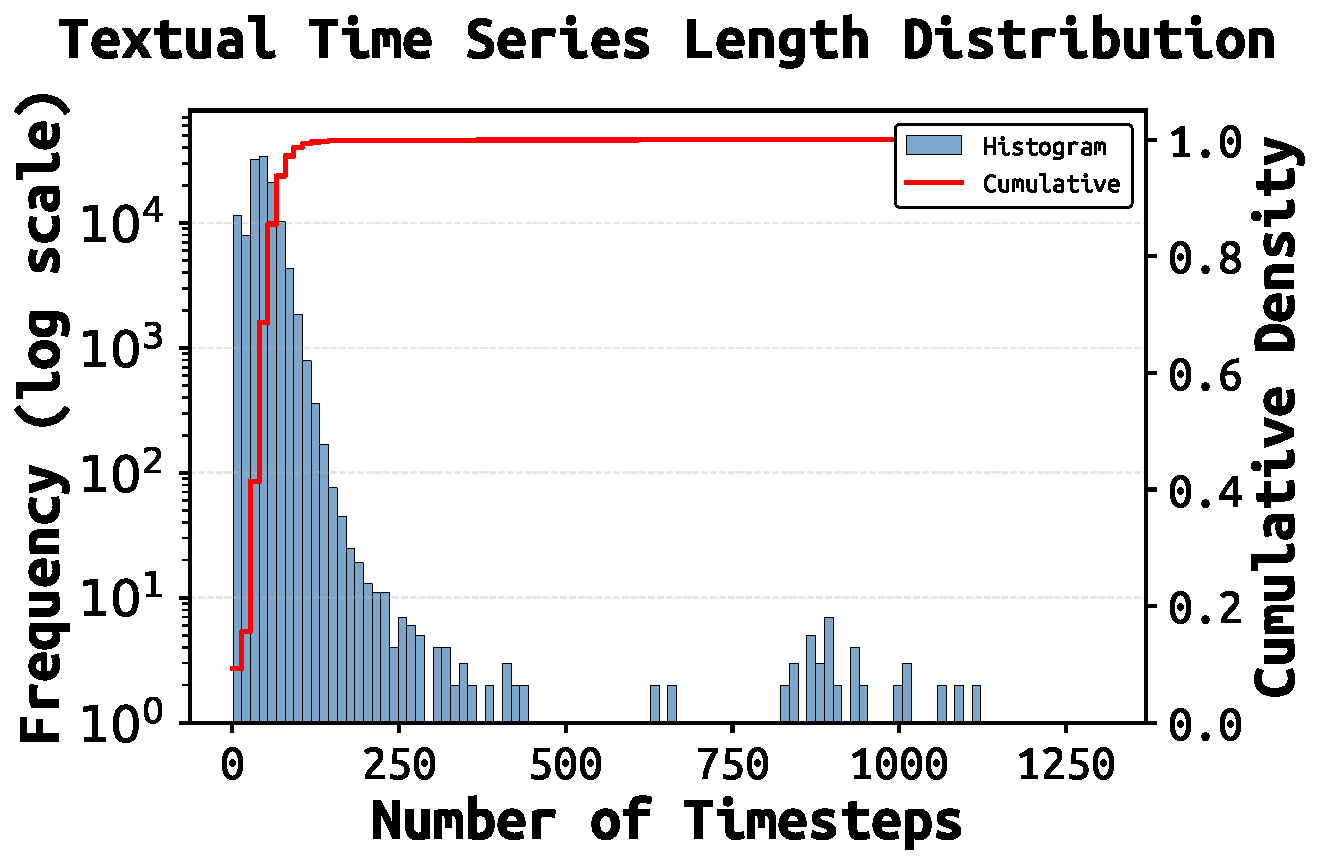
\includegraphics[width=\linewidth]{Chapters/chapter-05/images/Scientific_data/Plots_tables/tts_length_distribution.pdf}
        \ChFivePanelText{(a) Distribution of time series lengths (timesteps) across the dataset.}
    \end{minipage}\hfill
    \begin{minipage}{0.48\textwidth}
        \centering
        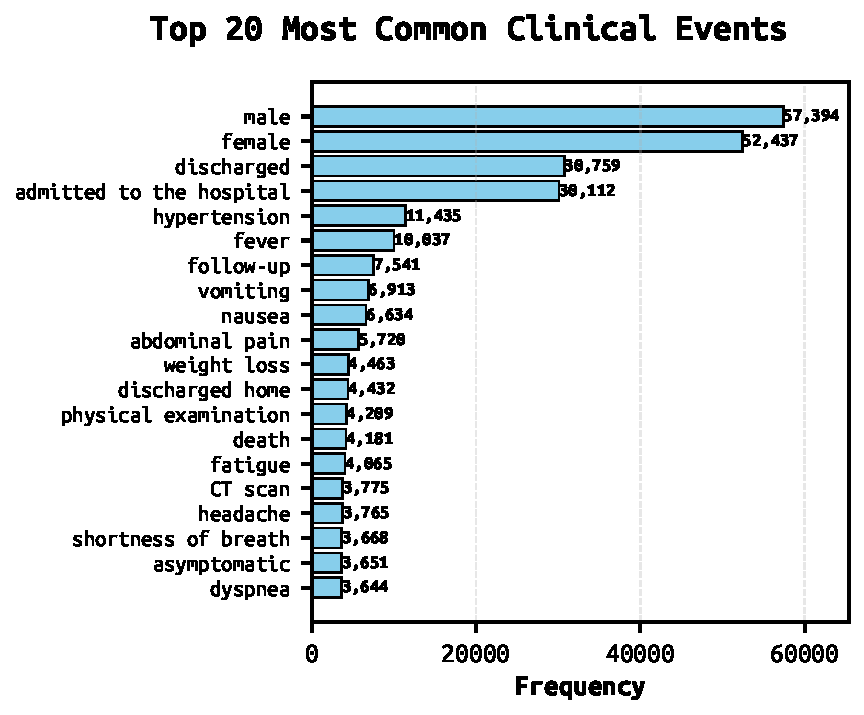
\includegraphics[width=\linewidth]{Chapters/chapter-05/images/Scientific_data/Plots_tables/top_20_common_events.pdf}
        \ChFivePanelText{(b) Most frequently occurring events across all case reports.
        }
    \end{minipage}
    
    
    % \vspace{-7.5mm}

\end{ChFiveFloatBody}
\caption{Overview of textual time series characteristics in PMOA-TTS.}\ChFiveFloatLabel{ch05:fig:tts_stats}
\end{figure}


